%% bare_jrnl.tex
%% V1.4b
%% 2015/08/26
%% by Michael Shell
%% see http://www.michaelshell.org/
%% for current contact information.
%%
%% This is a skeleton file demonstrating the use of IEEEtran.cls
%% (requires IEEEtran.cls version 1.8b or later) with an IEEE
%% journal paper.
%%
%% Support sites:
%% http://www.michaelshell.org/tex/ieeetran/
%% http://www.ctan.org/pkg/ieeetran
%% and
%% http://www.ieee.org/

%%*************************************************************************
%% Legal Notice:
%% This code is offered as-is without any warranty either expressed or
%% implied; without even the implied warranty of MERCHANTABILITY or
%% FITNESS FOR A PARTICULAR PURPOSE!
%% User assumes all risk.
%% In no event shall the IEEE or any contributor to this code be liable for
%% any damages or losses, including, but not limited to, incidental,
%% consequential, or any other damages, resulting from the use or misuse
%% of any information contained here.
%%
%% All comments are the opinions of their respective authors and are not
%% necessarily endorsed by the IEEE.
%%
%% This work is distributed under the LaTeX Project Public License (LPPL)
%% ( http://www.latex-project.org/ ) version 1.3, and may be freely used,
%% distributed and modified. A copy of the LPPL, version 1.3, is included
%% in the base LaTeX documentation of all distributions of LaTeX released
%% 2003/12/01 or later.
%% Retain all contribution notices and credits.
%% ** Modified files should be clearly indicated as such, including  **
%% ** renaming them and changing author support contact information. **
%%*************************************************************************


% *** Authors should verify (and, if needed, correct) their LaTeX system  ***
% *** with the testflow diagnostic prior to trusting their LaTeX platform ***
% *** with production work. The IEEE's font choices and paper sizes can   ***
% *** trigger bugs that do not appear when using other class files.       ***                          ***
% The testflow support page is at:
% http://www.michaelshell.org/tex/testflow/



\documentclass[journal]{IEEEtran}
%
% If IEEEtran.cls has not been installed into the LaTeX system files,
% manually specify the path to it like:
% \documentclass[journal]{../sty/IEEEtran}



% Some very useful LaTeX packages include:
% (uncomment the ones you want to load)


% *** MISC UTILITY PACKAGES ***
%
%\usepackage{ifpdf}
% Heiko Oberdiek's ifpdf.sty is very useful if you need conditional
% compilation based on whether the output is pdf or dvi.
% usage:
% \ifpdf
%   % pdf code
% \else
%   % dvi code
% \fi
% The latest version of ifpdf.sty can be obtained from:
% http://www.ctan.org/pkg/ifpdf
% Also, note that IEEEtran.cls V1.7 and later provides a builtin
% \ifCLASSINFOpdf conditional that works the same way.
% When switching from latex to pdflatex and vice-versa, the compiler may
% have to be run twice to clear warning/error messages.





% *** CITATION PACKAGES ***
%
%\usepackage{cite}
% cite.sty was written by Donald Arseneau
% V1.6 and later of IEEEtran pre-defines the format of the cite.sty package
% \cite{} output to follow that of the IEEE. Loading the cite package will
% result in citation numbers being automatically sorted and properly
% "compressed/ranged". e.g., [1], [9], [2], [7], [5], [6] without using
% cite.sty will become [1], [2], [5]--[7], [9] using cite.sty. cite.sty's
% \cite will automatically add leading space, if needed. Use cite.sty's
% noadjust option (cite.sty V3.8 and later) if you want to turn this off
% such as if a citation ever needs to be enclosed in parenthesis.
% cite.sty is already installed on most LaTeX systems. Be sure and use
% version 5.0 (2009-03-20) and later if using hyperref.sty.
% The latest version can be obtained at:
% http://www.ctan.org/pkg/cite
% The documentation is contained in the cite.sty file itself.






% *** GRAPHICS RELATED PACKAGES ***
%
\ifCLASSINFOpdf
  \usepackage[pdftex]{graphicx}
  % declare the path(s) where your graphic files are
  % \graphicspath{{../pdf/}{../jpeg/}}
  % and their extensions so you won't have to specify these with
  % every instance of \includegraphics
  % \DeclareGraphicsExtensions{.pdf,.jpeg,.png}
\else
  % or other class option (dvipsone, dvipdf, if not using dvips). graphicx
  % will default to the driver specified in the system graphics.cfg if no
  % driver is specified.
  % \usepackage[dvips]{graphicx}
  % declare the path(s) where your graphic files are
  % \graphicspath{{../eps/}}
  % and their extensions so you won't have to specify these with
  % every instance of \includegraphics
  % \DeclareGraphicsExtensions{.eps}
\fi
% graphicx was written by David Carlisle and Sebastian Rahtz. It is
% required if you want graphics, photos, etc. graphicx.sty is already
% installed on most LaTeX systems. The latest version and documentation
% can be obtained at:
% http://www.ctan.org/pkg/graphicx
% Another good source of documentation is "Using Imported Graphics in
% LaTeX2e" by Keith Reckdahl which can be found at:
% http://www.ctan.org/pkg/epslatex
%
% latex, and pdflatex in dvi mode, support graphics in encapsulated
% postscript (.eps) format. pdflatex in pdf mode supports graphics
% in .pdf, .jpeg, .png and .mps (metapost) formats. Users should ensure
% that all non-photo figures use a vector format (.eps, .pdf, .mps) and
% not a bitmapped formats (.jpeg, .png). The IEEE frowns on bitmapped formats
% which can result in "jaggedy"/blurry rendering of lines and letters as
% well as large increases in file sizes.
%
% You can find documentation about the pdfTeX application at:
% http://www.tug.org/applications/pdftex


\usepackage[framemethod=TikZ]{mdframed}
\usepackage{booktabs}
\usepackage[table]{xcolor}

% ===========================================================================================
% TIKZ PACKAGES AND CONFIGURATION
% ===========================================================================================
\usepackage{tikz}
\usepackage{pgfplots}
\pgfplotsset{compat=1.9}

% TikZ Libraries
\usetikzlibrary{patterns}
\usetikzlibrary{positioning}
\usetikzlibrary{fit}
\usetikzlibrary{calc}

% ===========================================================================================
% COLOR DEFINITIONS FOR CHARTS
% ===========================================================================================
\definecolor{rosso}{RGB}{220,57,18}
\definecolor{giallo}{RGB}{255,153,0}
\definecolor{blu}{RGB}{102,140,217}
\definecolor{verde}{RGB}{16,150,24}
\definecolor{viola}{RGB}{153,0,153}
\definecolor{hardblue}{RGB}{51,102,204}

% ===========================================================================================
% TIKZ STYLES FOR PIE CHARTS
% ===========================================================================================
\tikzset{
  chart/.style={
    legend label/.style={font={\scriptsize},anchor=west,align=left},
    legend box/.style={rectangle, draw, minimum size=10pt},
    axis/.style={black,semithick,->},
    axis label/.style={anchor=east,font={\tiny}},
  },
  pie chart/.style={
    chart,
    slice/.style={line cap=round, line join=round, very thick,draw=white},
    pie title/.style={font={\bfseries}},
    slice type/.style n args={3}{
        ##1/.style={pattern color=##2,pattern=##3},
        values of ##1/.style={
            black,
            font=\footnotesize,
            text opacity=1,
            fill=white,
            fill opacity=0.5,
            outer sep=\pgflinewidth
        }
    }
  }
}

% Layers for pie charts
\pgfdeclarelayer{background}
\pgfdeclarelayer{foreground}
\pgfsetlayers{background,main,foreground}

% Pie chart command
\newcommand{\pie}[3][]{
    \begin{scope}[#1]
    \pgfmathsetmacro{\curA}{90}
    \pgfmathsetmacro{\r}{1}
    \def\c{(0,0)}
    \def\offset{0}
    \foreach \v/\s/\number in{#3}{
        \pgfmathsetmacro{\deltaA}{\v/100*360}
        \pgfmathsetmacro{\nextA}{\curA + \deltaA}
        \pgfmathsetmacro{\midA}{(\curA+\nextA)/2}

        \path[slice,\s] \c
            -- +(\curA:\r)
            arc (\curA:\nextA:\r)
            -- cycle;
        \pgfmathsetmacro{\d}{max((\deltaA * -(.5/50) + 1) , .5)}

        \begin{pgfonlayer}{foreground}
        \path \c -- node[pos=\d+\offset,pie values,values of \s]{\number\hspace{.8mm}($\v\%$)} +(\midA:\r);
        \end{pgfonlayer}

        \global\let\curA\nextA
    }
    \end{scope}
}

% Legend command
\newcommand{\legendchart}[2][]{
    \begin{scope}[#1]
    \path
        \foreach \n/\s in {#2}
        {
            ++(0,-4pt) node[\s,legend box] {} +(2pt,0) node[legend label] {\n}
        }
    ;
    \end{scope}
}



% *** MATH PACKAGES ***
%
%\usepackage{amsmath}
% A popular package from the American Mathematical Society that provides
% many useful and powerful commands for dealing with mathematics.
%
% Note that the amsmath package sets \interdisplaylinepenalty to 10000
% thus preventing page breaks from occurring within multiline equations. Use:
%\interdisplaylinepenalty=2500
% after loading amsmath to restore such page breaks as IEEEtran.cls normally
% does. amsmath.sty is already installed on most LaTeX systems. The latest
% version and documentation can be obtained at:
% http://www.ctan.org/pkg/amsmath





% *** SPECIALIZED LIST PACKAGES ***
%
%\usepackage{algorithmic}
% algorithmic.sty was written by Peter Williams and Rogerio Brito.
% This package provides an algorithmic environment fo describing algorithms.
% You can use the algorithmic environment in-text or within a figure
% environment to provide for a floating algorithm. Do NOT use the algorithm
% floating environment provided by algorithm.sty (by the same authors) or
% algorithm2e.sty (by Christophe Fiorio) as the IEEE does not use dedicated
% algorithm float types and packages that provide these will not provide
% correct IEEE style captions. The latest version and documentation of
% algorithmic.sty can be obtained at:
% http://www.ctan.org/pkg/algorithms
% Also of interest may be the (relatively newer and more customizable)
% algorithmicx.sty package by Szasz Janos:
% http://www.ctan.org/pkg/algorithmicx

\usepackage{enumitem}


% *** ALIGNMENT PACKAGES ***
%
%\usepackage{array}
% Frank Mittelbach's and David Carlisle's array.sty patches and improves
% the standard LaTeX2e array and tabular environments to provide better
% appearance and additional user controls. As the default LaTeX2e table
% generation code is lacking to the point of almost being broken with
% respect to the quality of the end results, all users are strongly
% advised to use an enhanced (at the very least that provided by array.sty)
% set of table tools. array.sty is already installed on most systems. The
% latest version and documentation can be obtained at:
% http://www.ctan.org/pkg/array


% IEEEtran contains the IEEEeqnarray family of commands that can be used to
% generate multiline equations as well as matrices, tables, etc., of high
% quality.




% *** SUBFIGURE PACKAGES ***
%\ifCLASSOPTIONcompsoc
%  \usepackage[caption=false,font=normalsize,labelfont=sf,textfont=sf]{subfig}
%\else
%  \usepackage[caption=false,font=footnotesize]{subfig}
%\fi
% subfig.sty, written by Steven Douglas Cochran, is the modern replacement
% for subfigure.sty, the latter of which is no longer maintained and is
% incompatible with some LaTeX packages including fixltx2e. However,
% subfig.sty requires and automatically loads Axel Sommerfeldt's caption.sty
% which will override IEEEtran.cls' handling of captions and this will result
% in non-IEEE style figure/table captions. To prevent this problem, be sure
% and invoke subfig.sty's "caption=false" package option (available since
% subfig.sty version 1.3, 2005/06/28) as this is will preserve IEEEtran.cls
% handling of captions.
% Note that the Computer Society format requires a larger sans serif font
% than the serif footnote size font used in traditional IEEE formatting
% and thus the need to invoke different subfig.sty package options depending
% on whether compsoc mode has been enabled.
%
% The latest version and documentation of subfig.sty can be obtained at:
% http://www.ctan.org/pkg/subfig




% *** FLOAT PACKAGES ***
%
%\usepackage{fixltx2e}
% fixltx2e, the successor to the earlier fix2col.sty, was written by
% Frank Mittelbach and David Carlisle. This package corrects a few problems
% in the LaTeX2e kernel, the most notable of which is that in current
% LaTeX2e releases, the ordering of single and double column floats is not
% guaranteed to be preserved. Thus, an unpatched LaTeX2e can allow a
% single column figure to be placed prior to an earlier double column
% figure.
% Be aware that LaTeX2e kernels dated 2015 and later have fixltx2e.sty's
% corrections already built into the system in which case a warning will
% be issued if an attempt is made to load fixltx2e.sty as it is no longer
% needed.
% The latest version and documentation can be found at:
% http://www.ctan.org/pkg/fixltx2e


%\usepackage{stfloats}
% stfloats.sty was written by Sigitas Tolusis. This package gives LaTeX2e
% the ability to do double column floats at the bottom of the page as well
% as the top. (e.g., "\begin{figure*}[!b]" is not normally possible in
% LaTeX2e). It also provides a command:
%\fnbelowfloat
% to enable the placement of footnotes below bottom floats (the standard
% LaTeX2e kernel puts them above bottom floats). This is an invasive package
% which rewrites many portions of the LaTeX2e float routines. It may not work
% with other packages that modify the LaTeX2e float routines. The latest
% version and documentation can be obtained at:
% http://www.ctan.org/pkg/stfloats
% Do not use the stfloats baselinefloat ability as the IEEE does not allow
% \baselineskip to stretch. Authors submitting work to the IEEE should note
% that the IEEE rarely uses double column equations and that authors should try
% to avoid such use. Do not be tempted to use the cuted.sty or midfloat.sty
% packages (also by Sigitas Tolusis) as the IEEE does not format its papers in
% such ways.
% Do not attempt to use stfloats with fixltx2e as they are incompatible.
% Instead, use Morten Hogholm'a dblfloatfix which combines the features
% of both fixltx2e and stfloats:
%
% \usepackage{dblfloatfix}
% The latest version can be found at:
% http://www.ctan.org/pkg/dblfloatfix




%\ifCLASSOPTIONcaptionsoff
%  \usepackage[nomarkers]{endfloat}
% \let\MYoriglatexcaption\caption
% \renewcommand{\caption}[2][\relax]{\MYoriglatexcaption[#2]{#2}}
%\fi
% endfloat.sty was written by James Darrell McCauley, Jeff Goldberg and
% Axel Sommerfeldt. This package may be useful when used in conjunction with
% IEEEtran.cls'  captionsoff option. Some IEEE journals/societies require that
% submissions have lists of figures/tables at the end of the paper and that
% figures/tables without any captions are placed on a page by themselves at
% the end of the document. If needed, the draftcls IEEEtran class option or
% \CLASSINPUTbaselinestretch interface can be used to increase the line
% spacing as well. Be sure and use the nomarkers option of endfloat to
% prevent endfloat from "marking" where the figures would have been placed
% in the text. The two hack lines of code above are a slight modification of
% that suggested by in the endfloat docs (section 8.4.1) to ensure that
% the full captions always appear in the list of figures/tables - even if
% the user used the short optional argument of \caption[]{}.
% IEEE papers do not typically make use of \caption[]'s optional argument,
% so this should not be an issue. A similar trick can be used to disable
% captions of packages such as subfig.sty that lack options to turn off
% the subcaptions:
% For subfig.sty:
% \let\MYorigsubfloat\subfloat
% \renewcommand{\subfloat}[2][\relax]{\MYorigsubfloat[]{#2}}
% However, the above trick will not work if both optional arguments of
% the \subfloat command are used. Furthermore, there needs to be a
% description of each subfigure *somewhere* and endfloat does not add
% subfigure captions to its list of figures. Thus, the best approach is to
% avoid the use of subfigure captions (many IEEE journals avoid them anyway)
% and instead reference/explain all the subfigures within the main caption.
% The latest version of endfloat.sty and its documentation can obtained at:
% http://www.ctan.org/pkg/endfloat
%
% The IEEEtran \ifCLASSOPTIONcaptionsoff conditional can also be used
% later in the document, say, to conditionally put the References on a
% page by themselves.




% *** PDF, URL AND HYPERLINK PACKAGES ***
%
\usepackage{url}
% url.sty was written by Donald Arseneau. It provides better support for
% handling and breaking URLs. url.sty is already installed on most LaTeX
% systems. The latest version and documentation can be obtained at:
% http://www.ctan.org/pkg/url
% Basically, \url{my_url_here}.




% *** Do not adjust lengths that control margins, column widths, etc. ***
% *** Do not use packages that alter fonts (such as pslatex).         ***
% There should be no need to do such things with IEEEtran.cls V1.6 and later.
% (Unless specifically asked to do so by the journal or conference you plan
% to submit to, of course. )


% correct bad hyphenation here
\hyphenation{op-tical net-works semi-conduc-tor}


\begin{document}
%
% paper title
% Titles are generally capitalized except for words such as a, an, and, as,
% at, but, by, for, in, nor, of, on, or, the, to and up, which are usually
% not capitalized unless they are the first or last word of the title.
% Linebreaks \\ can be used within to get better formatting as desired.
% Do not put math or special symbols in the title.
\title{Bare Demo of IEEEtran.cls\\ for IEEE Journals}
%
%
% author names and IEEE memberships
% note positions of commas and nonbreaking spaces ( ~ ) LaTeX will not break
% a structure at a ~ so this keeps an author's name from being broken across
% two lines.
% use \thanks{} to gain access to the first footnote area
% a separate \thanks must be used for each paragraph as LaTeX2e's \thanks
% was not built to handle multiple paragraphs
%

\author{Rafael~Ribeiro,~\IEEEmembership{Mestrando,~UNIPAMPA,}
        John~Doe,~\IEEEmembership{Fellow,~OSA,}
        and~Jane~Doe,~\IEEEmembership{Life~Fellow,~IEEE}% <-this % stops a space
\thanks{M. Shell was with the Department
of Electrical and Computer Engineering, Georgia Institute of Technology, Atlanta,
GA, 30332 USA e-mail: (see http://www.michaelshell.org/contact.html).}% <-this % stops a space
\thanks{J. Doe and J. Doe are with Anonymous University.}% <-this % stops a space
\thanks{Manuscript received April 19, 2005; revised August 26, 2015.}}

% note the % following the last \IEEEmembership and also \thanks -
% these prevent an unwanted space from occurring between the last author name
% and the end of the author line. i.e., if you had this:
%
% \author{....lastname \thanks{...} \thanks{...} }
%                     ^------------^------------^----Do not want these spaces!
%
% a space would be appended to the last name and could cause every name on that
% line to be shifted left slightly. This is one of those "LaTeX things". For
% instance, "\textbf{A} \textbf{B}" will typeset as "A B" not "AB". To get
% "AB" then you have to do: "\textbf{A}\textbf{B}"
% \thanks is no different in this regard, so shield the last } of each \thanks
% that ends a line with a % and do not let a space in before the next \thanks.
% Spaces after \IEEEmembership other than the last one are OK (and needed) as
% you are supposed to have spaces between the names. For what it is worth,
% this is a minor point as most people would not even notice if the said evil
% space somehow managed to creep in.



% The paper headers
\markboth{Journal of \LaTeX\ Class Files,~Vol.~14, No.~8, August~2015}%
{Shell \MakeLowercase{\textit{et al.}}: Bare Demo of IEEEtran.cls for IEEE Journals}
% The only time the second header will appear is for the odd numbered pages
% after the title page when using the twoside option.
%
% *** Note that you probably will NOT want to include the author's ***
% *** name in the headers of peer review papers.                   ***
% You can use \ifCLASSOPTIONpeerreview for conditional compilation here if
% you desire.




% If you want to put a publisher's ID mark on the page you can do it like
% this:
%\IEEEpubid{0000--0000/00\$00.00~\copyright~2015 IEEE}
% Remember, if you use this you must call \IEEEpubidadjcol in the second
% column for its text to clear the IEEEpubid mark.



% use for special paper notices
%\IEEEspecialpapernotice{(Invited Paper)}




% make the title area
\maketitle

% As a general rule, do not put math, special symbols or citations
% in the abstract or keywords.
\begin{abstract}
    \textbf{Context}: In the software lifecycle, the market introduction phase presents significant challenges related to business model definition and selection. This raises questions such as which business models are available, which are most commonly adopted, which best fit the proposed solution, what benefits and limitations they present, and how to choose the most appropriate model.
    \textbf{Objective}: This study aims to map and categorize software business models, providing a structured view that supports understanding, comparison, and strategic selection.
    \textbf{Method}: A Systematic Literature Review (SLR) was conducted using primary studies from the last decade (2014--2024) indexed in the ACM, IEEE Xplore, and Scopus digital libraries. Data extraction employed 33 extraction questions (12 closed-ended and 21 open-ended), with qualitative analysis using a coding scheme of 61 codes organized in 9 classes.
    \textbf{Results}: The search retrieved 2,889 studies, with 216 removed as duplicates. After title and abstract screening, 312 studies were considered potentially relevant, and the full-text quality assessment resulted in 67 studies included in the final synthesis. The analysis identified platform-based models (391 mentions), SaaS (289), freemium (264), and open source (188) as the most prevalent. Subscription-based revenue dominated at 76.1\%, with multi-tenant SaaS present in 71.6\% of studies. Key success factors include ecosystem management (138 mentions) and market expansion (84), while main challenges involve security concerns (41) and revenue stream transformation (38).
    \textbf{Conclusion}: The consolidated results provide a three-dimensional taxonomy (delivery, monetization, ecosystem) and serve as conceptual foundation for developing an ontology to represent software business models, contributing to the systematization of knowledge and supporting evidence-based strategic decision-making.
\end{abstract}

% Note that keywords are not normally used for peerreview papers.
\begin{IEEEkeywords}
Business Model, Software, Systematic Literature Review.
\end{IEEEkeywords}






% For peer review papers, you can put extra information on the cover
% page as needed:
% \ifCLASSOPTIONpeerreview
% \begin{center} \bfseries EDICS Category: 3-BBND \end{center}
% \fi
%
% For peerreview papers, this IEEEtran command inserts a page break and
% creates the second title. It will be ignored for other modes.
\IEEEpeerreviewmaketitle



\section{Introduction}\label{sec:intro}
% The very first letter is a 2 line initial drop letter followed
% by the rest of the first word in caps.
%
% form to use if the first word consists of a single letter:
% \IEEEPARstart{A}{demo} file is ....
%
% form to use if you need the single drop letter followed by
% normal text (unknown if ever used by the IEEE):
% \IEEEPARstart{A}{}demo file is ....
%
% Some journals put the first two words in caps:
% \IEEEPARstart{T}{his demo} file is ....
%
% Here we have the typical use of a "T" for an initial drop letter
% and "HIS" in caps to complete the first word.
\IEEEPARstart{S}{oftware} development is a dynamic process that extends beyond code creation or feature delivery. In the software lifecycle, the market introduction phase presents itself as a crucial moment, where decisions related to monetization and financial sustainability must be carefully planned. In this context, business modeling plays a central role, providing frameworks to align the organization's strategic objectives with market needs.
% You must have at least 2 lines in the paragraph with the drop letter
% (should never be an issue)

Different business models, such as licensing, the freemium model, or Software as a Service (SaaS), have been widely explored in the software industry. However, choosing the most suitable model for a specific product involves considering various factors, such as market trends, implementation challenges, and effective practices for risk mitigation. Furthermore, the literature on business models often addresses varied aspects, making it difficult to identify emerging and successful approaches in the sector.

Given this complexity, this study aims to explore business models applied to the software industry through a systematic literature review (SLR) of the last 10 years (2014--2024). The research seeks to answer fundamental questions about which models have been used, which factors influence their selection, and which practices have been effective in overcoming implementation challenges. To this end, rigorous criteria were defined for selection, evaluation, and data extraction, ensuring the quality and relevance of the analyzed studies.

The results of this work aim to contribute to the creation of an ontology that supports both researchers and practitioners in the selection and implementation of effective business models for software products. By understanding the characteristics, success factors, and challenges of each approach, this study provides valuable insights for strategic decisions in the software industry.

The remainder of this article is organized as follows: Section~\ref{sec:methodology} presents the methodology used, including the research questions, selection criteria, and extraction strategy; Section~\ref{sec:analysis} presents the analysis of results organized by research question; Section~\ref{sec:discussion} discusses the main findings and their implications; Section~\ref{sec:threats} addresses threats to validity; and Section~\ref{sec:conclusion} presents conclusions and future work.






% TODO: Write Theoretical Foundation section - Include theoretical concepts about software business models,
% Business Model Canvas, value creation, monetization strategies, and platform economics.
% Add references to seminal works (Osterwalder, Teece, Parker/Van Alstyne, etc.)
\section{Theoretical Foundation}





% TODO: Write Related Work section - Review previous SLRs on software business models,
% compare methodologies and findings, identify gaps that this study addresses.
% Add references to related systematic reviews and mapping studies.
\section{Related Work}





\section{Methodology}\label{sec:methodology}
    \IEEEPARstart{S}{everal} guidelines have been proposed for conducting Systematic Literature Reviews (SLR) and Systematic Mapping Studies (SMS), such as those presented by \cite{keele2007guidelines}, \cite{engstrom2011software}, and \cite{petersen2008systematic}.
    This study primarily followed the guidelines described by \cite{petersen2008systematic}, which establish a structured process to identify research gaps, classify, and map the retrieved articles.
    According to the authors, systematic mapping should follow the process illustrated in Figure~\ref{fig:protocol}.

    \begin{figure}[!htb]
        \centering
        \includegraphics[width=3.2in]{img/protocol.png}
        \caption{Systematic Mapping Process \cite{petersen2008systematic}}
        \label{fig:protocol}
    \end{figure}

    The first step of the process consists of defining the research questions, enabling the identification of keywords for database searches. Subsequently, articles that do not meet the inclusion criteria, defined based on the research questions, are filtered out. The remaining articles are classified based on keywords found, especially in the abstracts. From the data extracted from the articles, a systematic map is constructed, which may include charts and tables to illustrate the results, as described by \cite{petersen2008systematic}.

\subsection{Research Questions}\label{sec:research-questions}

The motivation of this study is to understand the business models currently employed for software product monetization.

Based on this motivation, we formulated the following Research Questions (RQ):

\begin{figure}[!htb]
    \centering
    \begin{mdframed}[roundcorner=7pt,backgroundcolor=gray!25]
    \begin{enumerate}[label=\textbf{RQ\arabic*.}]
        \small
        \item \textbf{Business Model Identification and Taxonomy}: What business models have been identified in the literature for software product monetization, and how are they defined, classified, and differentiated from each other?\label{rq:01}
        \item \textbf{Application Context and Market Segmentation}: In which application contexts (vertical segments, customer types, geographies, and company sizes) have different software business models been implemented, and what segmentation patterns emerge from this distribution?\label{rq:02}
        \item \textbf{Technical and Architectural Characteristics}: What are the technical, architectural, and delivery characteristics that distinguish different software business models, and how do these characteristics influence monetization?\label{rq:03}
        \item \textbf{Monetization and Pricing Strategies}: What are the monetization and pricing strategies used in different software business models, and how do these strategies relate to the characteristics of the model and the market?\label{rq:04}
        \item \textbf{Ecosystem Dynamics and Go-to-Market}: What are the ecosystem dynamics (roles, relationships, network effects) and go-to-market strategies (acquisition channels, marketplaces) associated with different software business models?\label{rq:05}
        \item \textbf{Motivations, Success Factors, and Adoption Conditions}: What are the motivations for adoption, the factors that contribute to success, and the necessary conditions (prerequisites) for successful implementation of different software business models?\label{rq:06}
        \item \textbf{Implementation Challenges and Mitigation}: What are the main challenges faced in implementing different software business models, and what effective practices have been used to mitigate these challenges?\label{rq:07}
        \item \textbf{Temporal Evolution and Future Trends}: What is the temporal evolution and maturity of the different software business models identified in the literature, and what are the future trends and projected evolution directions?\label{rq:08}
        \item \textbf{Business Model Canvas Elements}: What are the distinctive characteristics and constituent elements (Business Model Canvas) of each identified software business model, and how do these elements relate to each other to create value?\label{rq:09}
        \item \textbf{Empirical Evidence and Methodologies}: What types of empirical evidence and research methodologies have been used to study software business models, and what are the patterns of available evidence for each model?\label{rq:10}
    \end{enumerate}
    \end{mdframed}
    \caption{Research Questions}
    \label{fig:RQs}
\end{figure}

These questions guided the search for relevant studies, enabling the identification of applied business models and contextual factors that influence the success of each approach.

The search strategy was developed based on terms related to the topic ``software business models'' and their synonyms. Thus, the following steps were adopted:
\begin{itemize}
    \item \textbf{Data Sources:} The databases selected for study collection were ACM Digital Library, IEEE Xplore, and Scopus;
    \item \textbf{Search Terms:} The terms ``Business model'' and ``Software'' were used, combined with Boolean operators to optimize results;
    \item \textbf{Search Period:} Studies published between 2014 and 2024 were considered, covering the last decade;
    \item \textbf{Language:} Only studies written in English were included in the research, ensuring uniformity in the analysis.
\end{itemize}

To expand the scope of the research, synonyms and related terms were identified and organized in Table~\ref{tab:terms-synonyms}. This table served as the basis for constructing the search string used in the databases.
The search string was elaborated using Boolean operators (\texttt{AND}, \texttt{OR}) to ensure precision and relevance of results.
The final formulation of the search string is presented in Figure~\ref{fig:String}.
The application of this search string to the databases resulted in the collection of studies aligned with the objectives of this work.

\rowcolors{1}{white}{gray!25}
\begin{table}[htbp]
    \caption{Terms and Synonyms}
    \label{tab:terms-synonyms}
    \centering
    \footnotesize
    \begin{tabular}{l|p{6cm}}
        \toprule
        \rowcolor{gray!50}
        \textbf{Term} & \textbf{Synonyms} \\
        \midrule
        \textit{Business model} & \textit{Revenue model}, \textit{Financial model}, \textit{Commercial proposal}, \textit{Monetization plan}, \textit{Subscription model}, \textit{Go-to-market strategy}, and \textit{Monetization strategy} \\
        \textit{Software} & \textit{App}, \textit{Information system}, \textit{SAAS} \\
        \bottomrule
    \end{tabular}
\end{table}


\begin{figure}[!htb]
    \centering
    \begin{mdframed}[roundcorner=7pt,backgroundcolor=gray!25]
    \centering
    \small
    \texttt{
    ("Business model" \textbf{OR} "Revenue model" \textbf{OR} "Financial model" \textbf{OR} "Commercial proposal" \textbf{OR} "Monetization plan" \textbf{OR} "Subscription model" \textbf{OR} "Go-to-market strategy" \textbf{OR} "Monetization strategy")
    \textbf{AND} ("Software" \textbf{OR} "App" \textbf{OR} "Information system" \textbf{OR} "SAAS")
    }
    \end{mdframed}
    \caption{Search String.}
    \label{fig:String}
\end{figure}

This approach ensured comprehensiveness and relevance in the selection of studies, enabling the identification of publications pertinent to the investigated topic.

\subsection{Study Selection Criteria}\label{sec:study-selection-criteria}
The selection criteria were established to ensure the relevance and quality of the studies included in the review:

\textbf{Inclusion Criteria (IC):}
    \begin{enumerate}[label=\textbf{IC\arabic*.}]
        \item \textbf{Access Availability:} Studies that are fully accessible for analysis;

        \item \textbf{Minimum Depth:} Studies with at least six pages, ensuring more detailed and well-founded discussions;

        \item \textbf{Focus on Software Business Models:} Studies that explicitly address business models applied to the software industry, including practical, theoretical, or hybrid approaches.
    \end{enumerate}

\textbf{Exclusion Criteria (EC):}
    \begin{enumerate}[label=\textbf{EC\arabic*.}]
        \item \textbf{Incomplete Documents:} Works with restricted access, extended abstracts, presentations, or posters;

        \item \textbf{Short Papers:} Works with fewer than six pages, as they do not present sufficient analytical depth;

        \item \textbf{Excessive Technical Focus:} Studies whose main topic is technical (such as architectures, algorithms, or software performance), in which business models play a secondary or irrelevant role.
    \end{enumerate}

\subsection{Study Quality Criteria}\label{sec:study-quality-criteria}
To assess the quality of the selected studies, the following Quality Questions (QQ) were defined, which serve as the basis for clarifying and applying the evaluation criteria:

\begin{enumerate}[label=\textbf{QQ\arabic*.}]
    \item Does the study present a specific business model for software? (Weight 4\label{qq:01})
    \item Does the study justify the choice of a business model based on relevant factors? (Weight 1\label{qq:02})
    \item Does the study identify business model(s) as emerging trends in recent literature? (Weight 1)
    \item Does the study discuss success factors and challenges faced by software companies in implementing business models? (Weight 1)
    \item Does the study present practices to mitigate challenges related to the implementation of software business models? (Weight 1\label{qq:05})
    \item Does the study describe in detail the characteristics of the analyzed business models? (Weight 2\label{qq:06})
\end{enumerate}

The quality assessment of studies was structured to prioritize information most relevant to the research objectives. Quality Question~\ref{qq:01} was defined as mandatory, as it is essential that each study analyze at least one business model applied to software. Quality Question~\ref{qq:06} also stands out, as it contributes a detailed description of the characteristics of the presented models. The remaining questions (\textbf{\ref{qq:02}--\ref{qq:05}}) are considered complementary and enrich the analysis, although their absence does not directly compromise the quality of the study in the review.

To classify studies based on their quality, weights were defined for each quality question and a scale that categorizes studies into six levels:

\begin{itemize}
    \item \textbf{Poor:} 0 to 0.99 points.
    \item \textbf{Weak:} 1 to 1.99 points.
    \item \textbf{Fair:} 2 to 3.99 points.
    \item \textbf{Good:} 4 to 5.99 points.
    \item \textbf{Very Good:} 6 to 7.99 points.
    \item \textbf{Excellent:} 8 to 10 points.
\end{itemize}

The final score of each study is calculated based on the weights assigned to each quality question, allowing for an objective and systematic evaluation. Thus, studies classified as ``Excellent'' are included in the final synthesis, ensuring greater relevance and depth to the research results.

\subsection{Data Extraction Strategy}\label{sec:data-extraction-strategy}

Data extraction was performed based on the previously defined research questions.
For this purpose, the following Extraction Questions (EQ) were used, which guide the collection and organization of relevant information:

\begin{enumerate}[label=\textbf{EQ\arabic*.}]
    \item Which software business models are presented in the study? (\ref{rq:01})
    \item Which factors were justified for choosing the business model? (\ref{rq:02})
    \item Is the presented business model indicated as an emerging trend? (\ref{rq:08})
    \item Which success factors are highlighted in the implementation of the business model by software companies? (\ref{rq:06})
    \item Which challenges are faced by software companies in implementing the business model? (\ref{rq:07})
    \item Which practices were indicated in the study to mitigate the challenges of business model implementation? (\ref{rq:07})
    \item What are the characteristics of each business model addressed in the study? (\ref{rq:03}, \ref{rq:04}, \ref{rq:09})
\end{enumerate}

\subsection{Extracted Data Synthesis}\label{sec:data-synthesis}

The data synthesis was performed qualitatively, seeking to answer the research questions. The results were organized in a thematic map, identifying:

\begin{itemize}
    \item \textbf{Business Model Categories:} An overview of the models identified in the studies;
    \item \textbf{Success Factors and Challenges:} A cross-analysis of factors that impact the success of models;
    \item \textbf{Emerging Trends:} Identification of new models and approaches adopted by software companies since 2014.
\end{itemize}

\subsection{Study Execution}\label{sec:execution}

The execution of this study began at the end of November 2024, following the protocol described and illustrated in Figure~\ref{fig:protocol}.
To support the planning and execution phases of the SMS, complementary tools were used.
The main tool employed was \textit{Thoth}, in its second version\footnote{\url{https://thoth-slr.com/}}.
However, since \textit{Thoth} was still under development and testing, \textit{Google Sheets}\footnote{\url{https://docs.google.com/spreadsheets/?usp=sheets_ald}} was used as an additional resource to ensure efficient data organization and management.

For all selected databases, the search was limited to the ``Abstract'' and ``Title'' fields to increase the precision of results and avoid irrelevant articles.
Additionally, date filters were applied directly in the databases, restricting the publication interval to the period from 2014 to 2024.

Figure~\ref{fig:papers-per-db} shows that the application of the search strategy resulted in the retrieval of 2,889 articles in total, distributed among the three selected databases: ACM Digital Library, IEEE Xplore, and Scopus.

\begin{figure}[!htb]
    \centering
    % ===========================================================================================
% Papers per Database - Pie Chart
% Dados: ACM (57, 2.0%), IEEE (225, 7.8%), Scopus (2607, 90.2%)
% Total: 2889 artigos
% ===========================================================================================
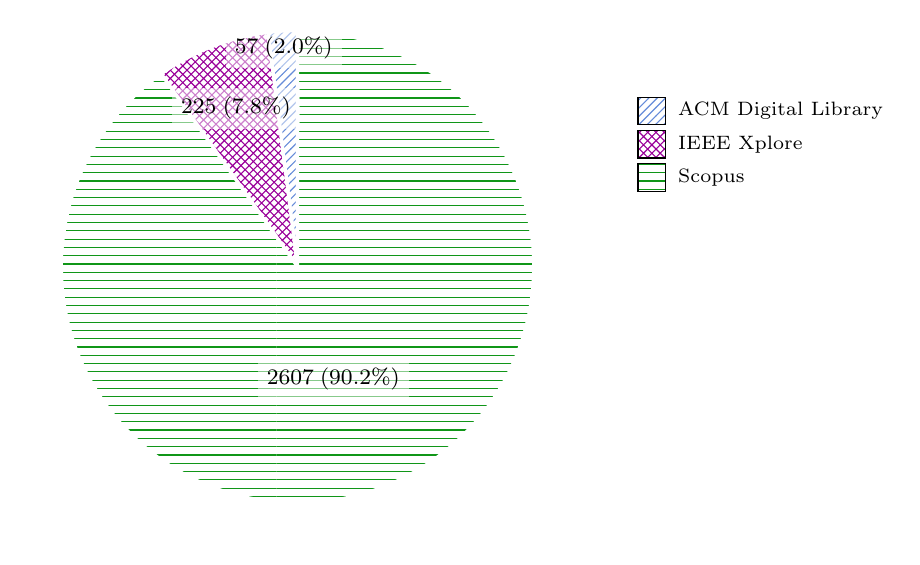
\begin{tikzpicture}
[
    pie chart,
    slice type={acm}{blu}{north east lines},
    slice type={ieee}{viola}{crosshatch},
    slice type={scopus}{verde}{horizontal lines},
    pie values/.style={font={\footnotesize}, fill=gray!0},
    scale=3
]
    \centering
    \pie{}{
        2.0/acm/57,
        7.8/ieee/225,
        90.2/scopus/2607}

    \legendchart[shift={(1.5cm,0.8cm)}]{
        {ACM Digital Library}/acm,
        {IEEE Xplore}/ieee,
        {Scopus}/scopus}
\end{tikzpicture}

    \caption{Studies per Database.}
    \label{fig:papers-per-db}
\end{figure}

\subsubsection{Study Selection}\label{sec:study-selection}
In the first phase of selection, 216 duplicate articles were identified and removed. Subsequently, the inclusion and exclusion criteria were applied through analysis of titles and abstracts. As a result of this screening, 312 studies were considered potentially relevant and selected for full-text reading in the next phase.

\subsubsection{Study Quality Assessment}\label{sec:quality-evaluation}
Of the 312 potentially relevant studies, 138 were submitted to full-text reading and quality assessment based on the Quality Questions (QQ) defined in Section~\ref{sec:study-quality-criteria}. After this rigorous analysis, 67 studies were classified as ``Excellent'' and accepted for inclusion in the final synthesis, fully meeting the established quality criteria and presenting relevant contributions to answer the research questions.

Figure~\ref{fig:quality-papers-evaluation} presents the distribution of the 138 studies according to the classification obtained in the quality assessment. Of the evaluated studies, 67 (48.6\%) were classified as ``Excellent'', 24 (17.4\%) as ``Very Good'', 3 (2.2\%) as ``Good'', 4 (2.9\%) as ``Fair'', 1 (0.7\%) as ``Weak'', and 39 (28.3\%) as ``Poor''.

\begin{figure}[!htb]
    \centering
    % ===========================================================================================
% Quality Classification of Studies - Pie Chart
% Study classification in quality assessment
% Total: 138 studies evaluated
% ===========================================================================================
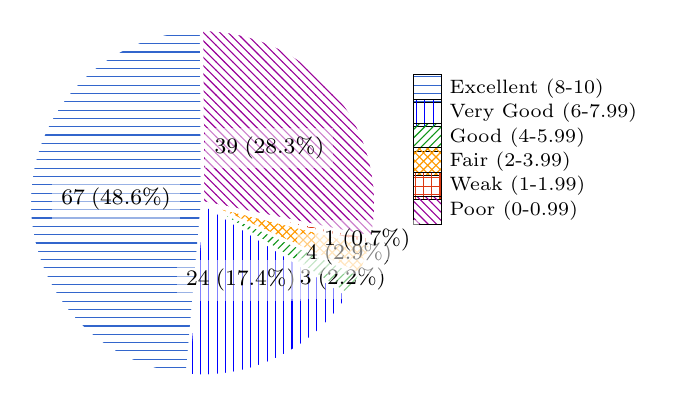
\begin{tikzpicture}
[
    pie chart,
    slice type={excelente}{hardblue}{horizontal lines},
    slice type={muitobom}{blue}{vertical lines},
    slice type={bom}{verde}{north east lines},
    slice type={regular}{giallo}{crosshatch},
    slice type={ruim}{rosso}{grid},
    slice type={pessimo}{viola}{north west lines},
    pie values/.style={font={\small}, fill=gray!0},
    scale=2.2
]
    \pie{}{
        48.6/excelente/67,
        17.4/muitobom/24,
        2.2/bom/3,
        2.9/regular/4,
        0.7/ruim/1,
        28.3/pessimo/39}

    \legendchart[shift={(1.3cm,0.8cm)}]{
        {Excellent (8-10)}/excelente,
        {Very Good (6-7.99)}/muitobom,
        {Good (4-5.99)}/bom,
        {Fair (2-3.99)}/regular,
        {Weak (1-1.99)}/ruim,
        {Poor (0-0.99)}/pessimo}
\end{tikzpicture}

    \caption{Study Classification in Quality Assessment.}
    \label{fig:quality-papers-evaluation}
\end{figure}

\subsubsection{Data Extraction}\label{sec:data-extraction}
Data extraction was performed on the 67 included studies, using a structured form with 33 extraction questions (EQ), organized into closed-ended questions (12 questions with predefined categories) and open-ended questions (21 questions for capturing qualitative information). The response rate varied according to the nature of the question: questions about model identification, application context, and success factors obtained rates close to 100\%, while more specific questions about licensing and billing periodicity presented lower rates (37--39\%), indicating that not all studies address these operational aspects.

For the qualitative analysis of open-ended questions, a coding scheme was developed with 61 codes organized into 9 classes and 35 subclasses, resulting in 4,630 quote classifications extracted from the studies. This coding process enabled the identification of patterns, categorization of recurring concepts, and establishment of relationships among the different aspects of the analyzed business models.





\section{Results Analysis}\label{sec:analysis}

This section presents the results of the analysis of the 67 studies included in the systematic review, organized according to the research questions defined in Section~\ref{sec:research-questions}.

\subsection{RQ1: Business Model Identification and Taxonomy}

The analysis of the studies enabled the identification of a diverse set of business models applied to the software industry. Table~\ref{tab:business-models-distribution} presents the main models identified and their frequency in the analyzed studies.

\begin{table}[!htb]
\renewcommand{\arraystretch}{1.3}
\caption{Distribuição dos Principais Modelos de Negócios Identificados}
\label{tab:business-models-distribution}
\centering
\small
\begin{tabular}{lrr}
\toprule
\textbf{Modelo de Negócio} & \textbf{Menções} & \textbf{\%} \\
\midrule
\rowcolor{gray!15} Platform business model & 391 & 8,4\% \\
SaaS (Software as a Service) & 289 & 6,2\% \\
\rowcolor{gray!15} Mobile app market & 279 & 6,0\% \\
Freemium model & 264 & 5,7\% \\
\rowcolor{gray!15} Open source business model & 188 & 4,1\% \\
B2B business model & 161 & 3,5\% \\
\rowcolor{gray!15} Subscription-based pricing & 153 & 3,3\% \\
Cloud delivery model & 152 & 3,3\% \\
\rowcolor{gray!15} Service-oriented model & 144 & 3,1\% \\
Network effects & 133 & 2,9\% \\
\midrule
\textbf{Total de classificações} & \textbf{4.630} & \textbf{100\%} \\
\bottomrule
\end{tabular}
\vspace{0.2cm}

\footnotesize\textit{Nota: Percentuais calculados sobre o total de 4.630 classificações de quotes. Um mesmo estudo pode mencionar múltiplos modelos.}
\end{table}


The Platform business model was the most frequently discussed, appearing in 391 mentions across the studies, followed by Software as a Service (SaaS) with 289 mentions. The mobile app market represented 279 mentions, evidencing the relevance of this segment. The Freemium model appeared in 264 mentions, demonstrating its popularity as a monetization strategy. Open source-based models were identified in 188 mentions.

Regarding delivery mode, 71.6\% of the studies mentioned the Multi-tenant SaaS model as the predominant form of software delivery. The cloud delivery model was referenced in 152 mentions, confirming the trend of migration to cloud-based infrastructures.

Concerning revenue sources, the Subscription model was identified as the main source in 76.1\% of the studies, followed by Usage/consumption (usage-based) with 41.8\% and Transaction (transactional) with 32.8\%. Advertising-based models represented 19.4\% of the studies, particularly relevant in mobile applications and freemium platforms. Figure~\ref{fig:revenue-sources} illustrates the distribution of identified revenue sources.

\begin{figure}[!htb]
    \centering
    % ===========================================================================================
% Revenue Sources - Horizontal Bar Chart
% Revenue sources identified in the studies
% Total: 67 studies
% ===========================================================================================
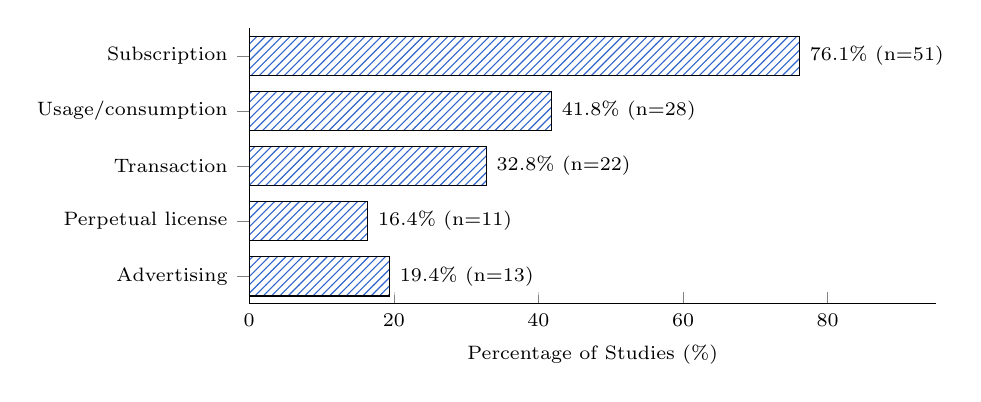
\begin{tikzpicture}
\begin{axis}[
    xbar,
    bar width=6pt,
    legend cell align=left,
    legend style={
        legend columns=1,
        at={(1.02,0.5)},
        anchor=west,
        draw=none,
        font=\scriptsize
    },
    ytick=data,
    axis y line*=none,
    axis x line*=bottom,
    x tick label style={font=\scriptsize},
    y tick label style={font=\scriptsize},
    label style={font=\scriptsize},
    xlabel={Percentage of Studies (\%)},
    xtick={0,20,40,60,80},
    xmin=0,
    xmax=95,
    width=0.85\columnwidth,
    height=4.5cm,
    bar width=5mm,
    yticklabels={
        {Advertising},
        {Perpetual license},
        {Transaction},
        {Usage/consumption},
        {Subscription}
    },
    area legend,
    y=7mm,
    enlarge y limits={abs=0.5},
    nodes near coords,
    nodes near coords align=horizontal,
    every node near coord/.append style={
        black,
        font=\scriptsize,
        text opacity=1,
        fill=white,
        fill opacity=0.6,
        outer sep=\pgflinewidth
    },
    visualization depends on={\thisrow{n} \as \mycount},
    nodes near coords={\pgfmathprintnumber\pgfplotspointmeta\% (n=\pgfmathprintnumber[fixed,precision=0]{\mycount})}
]
\addplot[pattern color=hardblue, pattern=north east lines] table [x=perc, y=idx, meta=perc] {
perc idx n
19.4 1 13
16.4 2 11
32.8 3 22
41.8 4 28
76.1 5 51
};
\end{axis}
\end{tikzpicture}

    \caption{Revenue Sources Identified in the Studies.}
    \label{fig:revenue-sources}
\end{figure}

\subsection{RQ2: Application Context and Market Segmentation}

The factors that influence the choice of monetization model can be categorized into: customer type, product/service type, acquisition channels, and network effects.

\subsubsection{Target Customer Type}

The analysis revealed that 53.7\% of the studies focused on Business-to-Business (B2B) models, while 41.8\% addressed Business-to-Consumer (B2C) models. The Enterprise segment was detailed in 7.5\% of the studies, while the focus on small and medium enterprises (SME) appeared in 35.8\%. Notably, many studies addressed multiple segments simultaneously, indicating the flexibility of software business models in serving different audiences. Figure~\ref{fig:customer-types} presents the distribution of target customer types.

\begin{figure}[!htb]
    \centering
    % ===========================================================================================
% Customer Types - Horizontal Bar Chart
% Target customer types identified in the studies
% Total: 67 studies
% ===========================================================================================
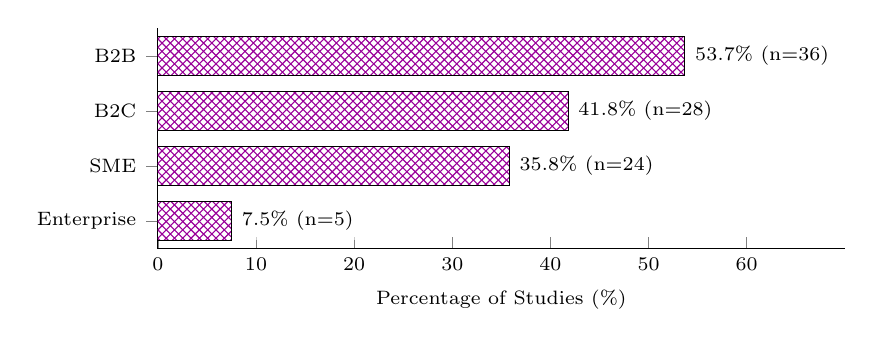
\begin{tikzpicture}
\begin{axis}[
    xbar,
    bar width=6pt,
    legend cell align=left,
    legend style={
        legend columns=1,
        at={(1.02,0.5)},
        anchor=west,
        draw=none,
        font=\scriptsize
    },
    ytick=data,
    axis y line*=none,
    axis x line*=bottom,
    x tick label style={font=\scriptsize},
    y tick label style={font=\scriptsize},
    label style={font=\scriptsize},
    xlabel={Percentage of Studies (\%)},
    xtick={0,10,20,30,40,50,60},
    xmin=0,
    xmax=70,
    width=0.85\columnwidth,
    height=4.5cm,
    bar width=5mm,
    yticklabels={
        {Enterprise},
        {SME},
        {B2C},
        {B2B}
    },
    area legend,
    y=7mm,
    enlarge y limits={abs=0.5},
    nodes near coords,
    nodes near coords align=horizontal,
    every node near coord/.append style={
        black,
        font=\scriptsize,
        text opacity=1,
        fill=white,
        fill opacity=0.6,
        outer sep=\pgflinewidth
    },
    visualization depends on={\thisrow{n} \as \mycount},
    nodes near coords={\pgfmathprintnumber\pgfplotspointmeta\% (n=\pgfmathprintnumber[fixed,precision=0]{\mycount})}
]
\addplot[pattern color=viola, pattern=crosshatch] table [x=perc, y=idx, meta=perc] {
perc idx n
7.5 1 5
35.8 2 24
41.8 3 28
53.7 4 36
};
\end{axis}
\end{tikzpicture}

    \caption{Identified Target Customer Types.}
    \label{fig:customer-types}
\end{figure}

\subsubsection{Product or Service Type}

Regarding offering type, 89.6\% of the studies addressed Applications (software applications), and 79.1\% addressed Platforms. Managed Services were discussed in 35.8\% of the studies, while Infrastructure represented 13.4\%. APIs were mentioned in 7.5\% of the studies as a form of value delivery.

\subsubsection{Customer Acquisition Channels}

The most frequent acquisition channels were: Direct sales in 47.8\% of the studies, Product-led Growth in 41.8\%, Partners/channels in 38.8\%, and Digital marketing in 37.3\%. The use of Marketplaces as a distribution channel was identified in 22.4\% of the studies. Figure~\ref{fig:customer-channels} presents the distribution of acquisition channels.

\begin{figure}[!htb]
    \centering
    % ===========================================================================================
% Customer Acquisition Channels - Horizontal Bar Chart
% Customer acquisition channels identified in the studies
% Total: 67 studies
% ===========================================================================================
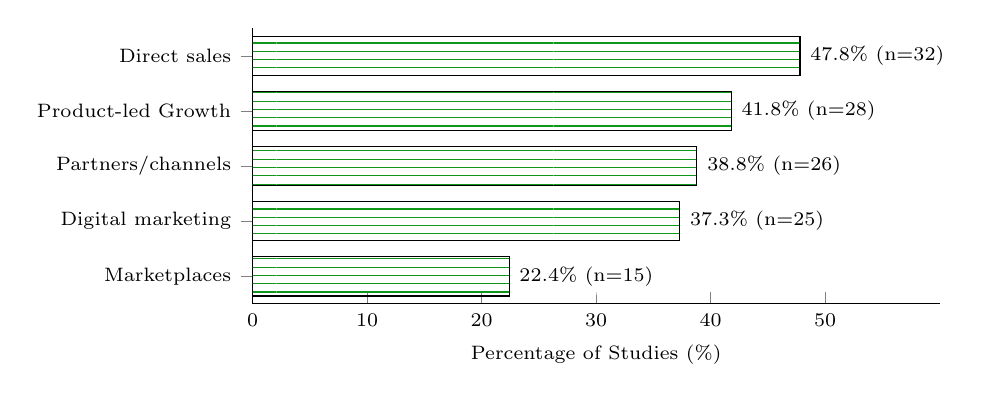
\begin{tikzpicture}
\begin{axis}[
    xbar,
    bar width=6pt,
    legend cell align=left,
    legend style={
        legend columns=1,
        at={(1.02,0.5)},
        anchor=west,
        draw=none,
        font=\scriptsize
    },
    ytick=data,
    axis y line*=none,
    axis x line*=bottom,
    x tick label style={font=\scriptsize},
    y tick label style={font=\scriptsize},
    label style={font=\scriptsize},
    xlabel={Percentage of Studies (\%)},
    xtick={0,10,20,30,40,50},
    xmin=0,
    xmax=60,
    width=0.85\columnwidth,
    height=5cm,
    bar width=5mm,
    yticklabels={
        {Marketplaces},
        {Digital marketing},
        {Partners/channels},
        {Product-led Growth},
        {Direct sales}
    },
    area legend,
    y=7mm,
    enlarge y limits={abs=0.5},
    nodes near coords,
    nodes near coords align=horizontal,
    every node near coord/.append style={
        black,
        font=\scriptsize,
        text opacity=1,
        fill=white,
        fill opacity=0.6,
        outer sep=\pgflinewidth
    },
    visualization depends on={\thisrow{n} \as \mycount},
    nodes near coords={\pgfmathprintnumber\pgfplotspointmeta\% (n=\pgfmathprintnumber[fixed,precision=0]{\mycount})}
]
\addplot[pattern color=verde, pattern=horizontal lines] table [x=perc, y=idx, meta=perc] {
perc idx n
22.4 1 15
37.3 2 25
38.8 3 26
41.8 4 28
47.8 5 32
};
\end{axis}
\end{tikzpicture}

    \caption{Customer Acquisition Channels.}
    \label{fig:customer-channels}
\end{figure}

\subsubsection{Network Effects}

Network effects were categorized into three main types: direct effects (Direct network effects---more users generate more value) in 35.8\% of the studies; cross-sided effects (Cross-sided effects---distinct groups benefit mutually) in 31.3\%; and data-based effects (Data network effects---more data improves the product) in 22.4\%. The presence of network effects was identified as a determining factor in the choice of platform and marketplace models. Figure~\ref{fig:network-effects} illustrates the distribution of network effect types.

\begin{figure}[!htb]
    \centering
    % ===========================================================================================
% Network Effects Types - Pie Chart
% Tipos de Efeitos de Rede identificados
% ===========================================================================================
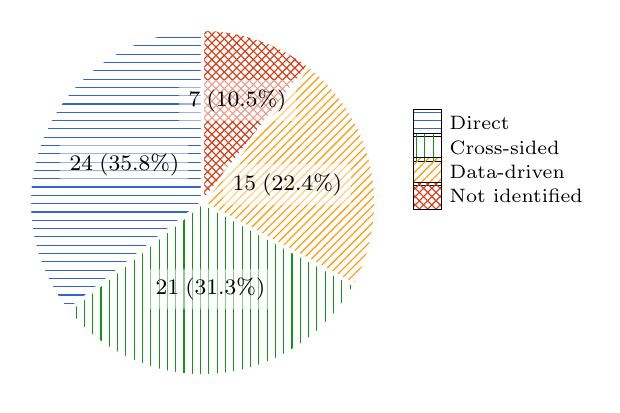
\begin{tikzpicture}
[
    pie chart,
    slice type={direct}{hardblue}{horizontal lines},
    slice type={cross}{verde}{vertical lines},
    slice type={data}{giallo}{north east lines},
    slice type={none}{rosso}{crosshatch},
    pie values/.style={font={\small}, fill=gray!0},
    scale=2.2
]
    \pie{}{
        35.8/direct/24,
        31.3/cross/21,
        22.4/data/15,
        10.5/none/7}

    \legendchart[shift={(1.3cm,0.6cm)}]{
        {Direct}/direct,
        {Cross-sided}/cross,
        {Data-driven}/data,
        {Not identified}/none}
\end{tikzpicture}

    \caption{Identified Network Effect Types.}
    \label{fig:network-effects}
\end{figure}

\subsection{RQ8: Temporal Evolution and Future Trends}

The temporal and thematic analysis of the studies revealed emerging trends in software business models. The Technology evolution code was identified in 83 mentions, indicating the importance of continuous technological adaptation. Future growth potential appeared in 49 mentions.

In terms of model maturity, 85 mentions were classified as growing business models, 80 as emerging business models, and 23 as consolidated business models.

Regarding the use of marketplaces and distribution platforms, the Apple App Store was mentioned in 20.9\% of the studies and the Google Play Store in 19.4\%, evidencing the dominance of mobile app stores. Enterprise cloud marketplaces (AWS, Azure, Google Cloud) still showed low penetration in the studies (3\% each), suggesting an area of growth.

Specific trends identified include: the integration of ecological sustainability in digital business models; the convergence between digital and sustainable transformation; the growth of Everything as a Service (XaaS) based models; and the increasing importance of data and artificial intelligence in value creation.

\subsection{RQ6 \& RQ7: Success Factors, Challenges, and Mitigation Practices}

\subsubsection{Success Factors}

The main success factors identified were organized into five categories:

\begin{enumerate}
    \item \textbf{Ecosystem management}: With 138 mentions, this was the most cited factor. It involves effective management of relationships with partners, developers, and stakeholders.

    \item \textbf{Market expansion}: Identified in 84 mentions, it refers to the strategy of expanding the customer base to achieve economies of scale.

    \item \textbf{Organizational preparedness}: With 64 mentions, it highlights the importance of the company's readiness to implement changes in the business model.

    \item \textbf{Service quality improvement}: Present in 36 mentions, it emphasizes the need for continuous improvement for customer retention.

    \item \textbf{Value-based orientation}: With 36 mentions, it represents the strategy of focusing on delivering customer-perceived value.
\end{enumerate}

Figure~\ref{fig:success-factors} presents the distribution of identified success factors.

\begin{figure}[!htb]
    \centering
    % ===========================================================================================
% Success Factors - Horizontal Bar Chart
% Fatores de Sucesso identificados na literatura
% ===========================================================================================
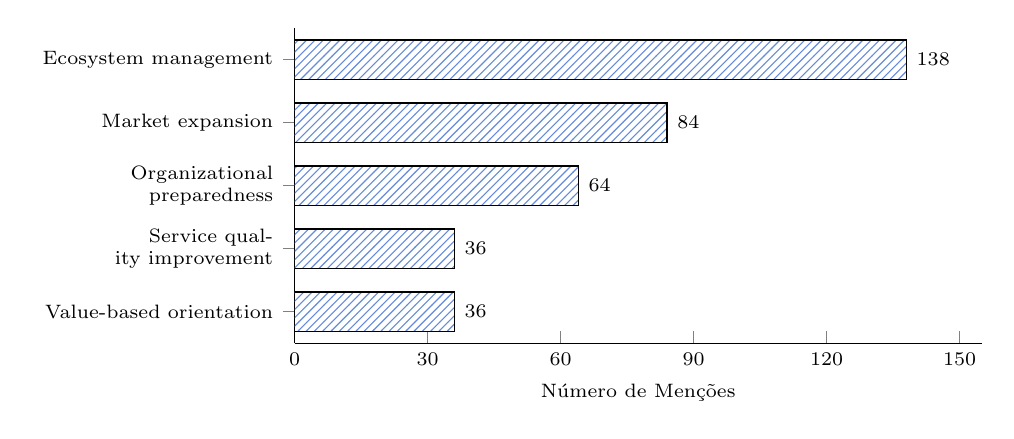
\begin{tikzpicture}
\begin{axis}[
    xbar,
    bar width=6pt,
    legend cell align=left,
    legend style={
        legend columns=1,
        at={(1.02,0.5)},
        anchor=west,
        draw=none,
        font=\scriptsize
    },
    ytick=data,
    axis y line*=none,
    axis x line*=bottom,
    x tick label style={font=\scriptsize},
    y tick label style={font=\scriptsize, text width=3cm, align=right},
    label style={font=\scriptsize},
    xlabel={Número de Menções},
    xtick={0,30,60,90,120,150},
    xmin=0,
    xmax=155,
    width=0.85\columnwidth,
    height=5cm,
    bar width=5mm,
    yticklabels={
        {Value-based orientation},
        {Service quality improvement},
        {Organizational preparedness},
        {Market expansion},
        {Ecosystem management}
    },
    area legend,
    y=8mm,
    enlarge y limits={abs=0.5},
    nodes near coords,
    nodes near coords align=horizontal,
    every node near coord/.append style={
        black,
        font=\scriptsize,
        text opacity=1,
        fill=white,
        fill opacity=0.6,
        outer sep=\pgflinewidth
    }
]
\addplot[pattern color=blu, pattern=north east lines] coordinates
{(36,1)(36,2)(64,3)(84,4)(138,5)};
\end{axis}
\end{tikzpicture}

    \caption{Success Factors in Business Model Implementation.}
    \label{fig:success-factors}
\end{figure}

\subsubsection{Implementation Challenges}

The main challenges identified were categorized according to Table~\ref{tab:implementation-challenges}:

\begin{table}[!htb]
\renewcommand{\arraystretch}{1.3}
\caption{Identified Implementation Challenges}
\label{tab:implementation-challenges}
\centering
\small
\begin{tabular}{p{4cm}p{2.5cm}r}
\toprule
\textbf{Challenge} & \textbf{Category} & \textbf{Mentions} \\
\midrule
\rowcolor{gray!15} Security concerns & Customer barriers & 41 \\
Revenue stream transformation & Financial impact & 38 \\
\rowcolor{gray!15} Organizational readiness & Customer barriers & 23 \\
Partner ecosystem disruption & Ecosystem impact & 23 \\
\rowcolor{gray!15} Customer trust maintenance & Customer barriers & 19 \\
Quality management & Operational impact & 15 \\
\midrule
\textbf{Total} & & \textbf{159} \\
\bottomrule
\end{tabular}
\vspace{0.2cm}

\footnotesize\textit{Note: Challenges identified through qualitative coding of open-ended questions.}
\end{table}


\begin{enumerate}
    \item \textbf{Security concerns}: With 41 mentions, this represents the main barrier identified by customers, especially in cloud-based models.

    \item \textbf{Revenue stream transformation}: Identified in 38 mentions, it refers to the challenge of migrating from one-time payments to recurring revenue models.

    \item \textbf{Organizational readiness}: With 23 mentions, it highlights the capability of customer organizations to adopt new business models.

    \item \textbf{Partner ecosystem disruption}: Present in 23 mentions, it evidences the impact of business model changes on relationships with partners and resellers.

    \item \textbf{Customer trust maintenance}: With 19 mentions, it represents the challenge of maintaining trust during business model transitions.
\end{enumerate}

\subsubsection{Mitigation Practices (RQ7 continued)}

The practices identified to mitigate implementation challenges were:

\begin{enumerate}
    \item \textbf{Flexible pricing strategies}: With 58 mentions, this was the most cited practice. It involves adapting pricing models to accommodate different customer needs and profiles.

    \item \textbf{Hybrid model adoption}: Identified in 13 mentions, it refers to the strategy of simultaneously maintaining old and new models during transition periods.

    \item \textbf{Pilot implementation}: With 8 mentions, it represents the approach of conducting controlled deployments with selected customers before large-scale adoption.

    \item \textbf{Partner compensation}: Present in 3 mentions, it involves financial support for partners affected by business model changes.
\end{enumerate}

\subsection{RQ3, RQ4, RQ5 \& RQ9: Business Model Characteristics}

The characteristics of business models were organized into dimensions according to the developed coding scheme. The Business model characteristics class concentrated 2,290 classified quotes, representing the highest density of extracted information.

\subsubsection{Pricing Strategies}

Four main strategies were identified:
\begin{itemize}
    \item \textbf{Subscription-based pricing} (153 mentions): Recurring payment model with monthly or annual billing for software access.
    \item \textbf{Pay-as-you-go pricing} (40 mentions): Consumption-based model where the customer pays for what they use.
    \item \textbf{Value-based pricing} (33 mentions): Pricing based on customer-perceived value.
    \item \textbf{Cost-based pricing} (15 mentions): Pricing based on vendor costs.
\end{itemize}

\subsubsection{Revenue Models}

The main revenue models identified were:
\begin{itemize}
    \item \textbf{Freemium model} (264 mentions): Offers a free basic version with paid premium features.
    \item \textbf{Open source business model} (188 mentions): Based on open source software with various commercialization strategies.
    \item \textbf{Data-driven monetization} (108 mentions): Revenue generation from data and analytics.
    \item \textbf{Perpetual licensing} (14 mentions): Traditional licensing model with one-time payment.
\end{itemize}

\subsubsection{Technical Architecture}

The technical infrastructure was characterized by:
\begin{itemize}
    \item \textbf{Cloud computing infrastructure} (95 mentions): Enabling infrastructure for cloud delivery.
    \item \textbf{Multi-tenant architecture} (24 mentions): Architecture where a single instance serves multiple customers.
    \item \textbf{On-demand access} (24 mentions): Software access available immediately when needed.
    \item \textbf{Remote hosting} (18 mentions): Software hosted on external servers.
\end{itemize}

\subsubsection{Value Creation}

Value creation mechanisms include:
\begin{itemize}
    \item \textbf{Platform business model} (391 mentions): Value creation through ecosystems of external connections.
    \item \textbf{Network effects} (133 mentions): Benefit where value increases with more users.
    \item \textbf{Marketplace model} (63 mentions): Facilitation of transactions between multiple parties.
\end{itemize}





\section{Discussion}\label{sec:discussion}

This section discusses the main findings of the systematic review, presenting an integrated synthesis of results and their implications for researchers and practitioners.

\subsection{Synthesis of Main Findings}

The analysis of 67 studies revealed a rich and diverse landscape of software business models. The predominance of the SaaS model (76.1\% of studies mentioning subscription as a revenue source) confirms the fundamental transformation that occurred in the software industry over the last decade. This model offers advantages both for vendors---predictable recurring revenue, piracy reduction, continuous update cycles---and for customers---lower initial investment, scalability, and access to constant updates.

The strong presence of platform models (391 mentions) and associated network effects (133 mentions) evidence the growing importance of ecosystems in the software market. Successful companies not only sell products but orchestrate ecosystems that connect developers, users, and partners, creating value through positive network effects.

The freemium model (264 mentions) emerged as a relevant strategy, particularly in B2C markets and mobile applications. This approach reduces entry barriers for users, allowing experimentation before conversion to paid versions. However, the studies indicate that freemium success depends on specific factor configurations, not being universally applicable.

\subsection{Identified Patterns and Correlations}

Cross-analysis of the data revealed important patterns:

\subsubsection{Correlation between Customer Type and Acquisition Channels}

B2B models tend to use direct sales (75\%) and channel partners (61\%), while B2C models favor Product-led Growth (68\%), digital marketing (54\%), and marketplaces (39\%). This differentiation reflects the distinct purchase journeys and decision-making processes of each segment.

\subsubsection{Correlation between Ecosystem Role and Network Effects}

Companies with a bilateral platform role (Two-sided platform) predominantly present cross-sided network effects (76\%), while standalone products show more varied distribution between direct effects (50\%) and absence of network effects (30\%).

\subsubsection{Evolution of Pricing Models}

The data indicate an evolution from perpetual licensing-based models (14 mentions) to subscription (153 mentions) and consumption (40 mentions) models. This transition represents a fundamental change in the relationship between vendors and customers, from single transaction to continuous relationship.

\subsection{Comparison with Prior Literature}

% TODO: Fix incorrect citation - \cite{keele2007guidelines} is about SLR guidelines (Kitchenham),
% NOT about network effects. Replace with appropriate reference on network effects
% (e.g., Parker/Van Alstyne, Katz/Shapiro, or Eisenmann on platform strategy).
The results of this review confirm and expand findings from previous studies on software business models. The predominance of SaaS corroborates the growth predictions identified in studies from the beginning of the decade. The importance of network effects, highlighted by \cite{keele2007guidelines}, was empirically confirmed, with more than one-third of the studies identifying some type of network effect.

The identification of challenges related to revenue stream transformation and partner ecosystem disruption adds detail to the existing literature on business model transitions. Prior literature frequently focused on the benefits of migrating to SaaS, while this review balances the perspective by systematically documenting the challenges faced.

\subsection{Emerging Taxonomy}

Based on the analysis, a taxonomy of software business models organized into three main dimensions is proposed:

\begin{enumerate}
    \item \textbf{Delivery Dimension}: How software is delivered (SaaS multi-tenant, single-tenant, on-premises, hybrid, mobile).

    \item \textbf{Monetization Dimension}: How revenue is generated (subscription, usage-based, freemium, perpetual license, advertising, transaction fees).

    \item \textbf{Ecosystem Dimension}: The company's role and value creation mechanisms (standalone product, two-sided platform, marketplace, plugin/complement).
\end{enumerate}

This taxonomy allows for systematic classification and comparison of software business models, facilitating the analysis of strategic options for companies in the sector.

\subsection{Implications for Practice}

For practitioners and managers of software companies, the results suggest:

\begin{enumerate}
    \item \textbf{Gradual transition strategy}: The adoption of hybrid models during transition periods reduces risks and allows adjustments based on market feedback.

    \item \textbf{Ecosystem investment}: Effective management of partners and stakeholders is the most cited success factor, indicating the need for investments in this area.

    \item \textbf{Pricing flexibility}: Flexible pricing strategies that accommodate different customer profiles are essential for maximizing adoption and revenue.

    \item \textbf{Security attention}: Security concerns are the main identified barrier, requiring investments in certifications, transparency, and communication.

    \item \textbf{Channel-customer alignment}: The choice of acquisition channels should be aligned with the target customer type (B2B vs. B2C).
\end{enumerate}

\subsection{Implications for Research}

For researchers, the findings indicate:

\begin{enumerate}
    \item \textbf{Gap in experimental studies}: Only 3\% of studies used experimental methods, indicating an opportunity for research that establishes causal relationships.

    \item \textbf{Underexploration of cloud marketplaces}: The low percentage of studies on AWS Marketplace, Azure Marketplace, and similar (3\% each) suggests an emerging area for investigation.

    \item \textbf{Need for longitudinal studies}: Most studies present cross-sectional views; longitudinal studies on business model evolution are necessary.

    \item \textbf{Integration with sustainability}: The emergence of sustainable digital business models represents a promising research frontier.
\end{enumerate}





\section{Threats to Validity}\label{sec:threats}

This section discusses the main threats to the validity of this study, organized according to the categories proposed by \cite{petersen2008systematic}.

\subsection{Construct Validity}

Construct validity refers to the adequacy of the measures used to capture the investigated concepts.

\textbf{Research question definition}: The research questions were defined based on prior literature reviews and validated through discussions among researchers. However, the breadth of the questions may have resulted in heterogeneous responses, making synthesis difficult.

\textbf{Extraction form}: The form with 33 extraction questions was developed iteratively and tested on a subset of studies before full application. Despite this, some questions presented low response rates (37--39\% for questions about licensing and billing periodicity), indicating possible misalignment between the questions and study content.

\textbf{Coding scheme}: The 61 codes used in qualitative analysis were developed iteratively through an inductive-deductive process. Coding validity was verified through cross-review of a sample of classifications.

\subsection{Internal Validity}

Internal validity refers to the reliability of study execution processes.

\textbf{Selection bias}: Study selection was performed following predefined criteria. However, the screening of 2,889 articles by a single researcher in the initial phase may have introduced bias. To mitigate this risk, doubtful cases were discussed with co-researchers.

\textbf{Extraction bias}: Data extraction was performed by one researcher, with sampling verification by a second researcher. The agreement rate was satisfactory, but occasional divergences may have occurred in ambiguous cases.

\textbf{Qualitative coding}: The assignment of codes to extracted quotes involved interpretive judgment. To increase reliability, detailed descriptions were developed for each code and periodic consistency reviews were conducted.

\subsection{External Validity}

External validity refers to the generalization of results.

\textbf{Temporal scope}: The study was limited to publications from 2014 to 2024, a period that captures SaaS model maturation but may not reflect more recent trends, such as generative artificial intelligence-based models.

\textbf{Database scope}: Three databases were used (ACM, IEEE Xplore, Scopus). Although representative of software engineering and information systems literature, studies published in other sources (management conferences, gray literature) may not have been captured.

\textbf{Publication bias}: Published studies tend to report positive or significant results, potentially under-representing failure experiences or neutral results in business model implementation.

\textbf{Geographic and industrial context}: The analyzed studies show predominance of North American and European contexts, and sectors such as mobile applications and enterprise platforms. Generalization to other contexts should be done with caution.

\subsection{Reliability}

Reliability refers to the possibility of study replication.

\textbf{Protocol documentation}: The research protocol was documented in detail, including search string, inclusion/exclusion criteria, and extraction questions. Raw data and analysis codes are available in a public repository for verification.

\textbf{Tools used}: The combined use of tools (Thoth and Google Sheets) for data management may hinder exact replication. However, procedures were documented to allow equivalent reproduction.

\subsection{Adopted Mitigations}

To mitigate the identified threats, the following strategies were adopted:

\begin{itemize}
    \item Prior definition and documentation of the research protocol;
    \item Iterative development of the extraction form with pilot testing;
    \item Creation of a hierarchical coding scheme with explicit definitions;
    \item Cross-review of selection, extraction, and coding samples;
    \item Availability of data and materials in an open repository;
    \item Triangulation of quantitative (closed-ended questions) and qualitative (open-ended questions) data.
\end{itemize}





\section{Conclusion}\label{sec:conclusion}

This study presented a systematic literature review on software business models, analyzing 67 studies published between 2014 and 2024. The research addressed the ten proposed research questions, contributing to the systematization of knowledge in the area.

\subsection{Main Contributions}

The main contributions of this work are:

\begin{enumerate}
    \item \textbf{Comprehensive mapping}: Identification and categorization of 61 codes organized into 9 classes, representing different aspects of software business models, from technical characteristics to success factors and challenges.

    \item \textbf{Quantitative evidence}: Consolidation of data on the prevalence of different models, highlighting SaaS/subscription (76.1\%), platforms (391 mentions), and freemium (264 mentions).

    \item \textbf{Model taxonomy}: Proposition of a three-dimensional taxonomy (delivery, monetization, ecosystem) for classifying software business models.

    \item \textbf{Synthesis of challenges and mitigations}: Systematic documentation of 159 mentions of implementation challenges and 82 mentions of mitigation practices.

    \item \textbf{Trend identification}: Mapping of emerging trends, including sustainability integration, data-based network effects, and platform-based models.
\end{enumerate}

\subsection{Answers to Research Questions}

\textbf{RQ1}: The most commonly used models are based on platforms, SaaS, freemium, and open source, with predominance of cloud delivery and subscription-based monetization.

\textbf{RQ2}: Models are implemented across diverse contexts, with 53.7\% focusing on B2B, 41.8\% on B2C, and varying distribution across vertical segments and company sizes.

\textbf{RQ3}: Technical characteristics include multi-tenant SaaS delivery (71.6\%), cloud infrastructure (95 mentions), multi-tenant architecture (24 mentions), and on-demand access (24 mentions).

\textbf{RQ4}: Monetization strategies include subscription (76.1\%), usage-based (41.8\%), and transaction-based (32.8\%), with pricing models varying from value-based to pay-as-you-go.

\textbf{RQ5}: Ecosystem dynamics involve platform roles (391 mentions), network effects (133 mentions), with go-to-market strategies including direct sales (47.8\%) and product-led growth (41.8\%).

\textbf{RQ6}: Main success factors are ecosystem management (138 mentions), market expansion (84), and organizational preparedness (64).

\textbf{RQ7}: Challenges include security concerns (41 mentions), revenue stream transformation (38), and partner disruption (23). Effective mitigation practices include flexible pricing strategies (58 mentions) and hybrid model adoption (13).

\textbf{RQ8}: Emerging trends include technology evolution (83 mentions), with 85 growing models and 80 emerging models identified.

\textbf{RQ9}: Models are characterized by delivery dimensions (SaaS multi-tenant, cloud), monetization dimensions (subscription, freemium), and ecosystem dimensions (platform, marketplace).

\textbf{RQ10}: Studies employ diverse methodologies, with predominance of case studies and empirical analyses, though experimental studies remain underrepresented (3\%).

\subsection{Future Work}

Based on the results and identified gaps, the following directions for future research are suggested:

\begin{itemize}
    \item Development of a formal ontology for representing software business models, enabling automated reasoning and decision support;

    \item Experimental studies that establish causal relationships between business model configurations and performance;

    \item In-depth investigation of business models based on artificial intelligence and machine learning;

    \item Longitudinal analysis of business model evolution in specific companies;

    \item Studies on the effectiveness of enterprise cloud marketplaces as a distribution channel.
\end{itemize}

The consolidated results of this systematic review provide a solid conceptual foundation for the development of tools and frameworks that support researchers and practitioners in understanding, comparing, and selecting business models for software products.

% An example of a floating figure using the graphicx package.
% Note that \label must occur AFTER (or within) \caption.
% For figures, \caption should occur after the \includegraphics.
% Note that IEEEtran v1.7 and later has special internal code that
% is designed to preserve the operation of \label within \caption
% even when the captionsoff option is in effect. However, because
% of issues like this, it may be the safest practice to put all your
% \label just after \caption rather than within \caption{}.
%
% Reminder: the "draftcls" or "draftclsnofoot", not "draft", class
% option should be used if it is desired that the figures are to be
% displayed while in draft mode.
%
%\begin{figure}[!t]
%\centering
%\includegraphics[width=2.5in]{myfigure}
% where an .eps filename suffix will be assumed under latex,
% and a .pdf suffix will be assumed for pdflatex; or what has been declared
% via \DeclareGraphicsExtensions.
%\caption{Simulation results for the network.}
%\label{fig_sim}
%\end{figure}

% Note that the IEEE typically puts floats only at the top, even when this
% results in a large percentage of a column being occupied by floats.


% An example of a double column floating figure using two subfigures.
% (The subfig.sty package must be loaded for this to work.)
% The subfigure \label commands are set within each subfloat command,
% and the \label for the overall figure must come after \caption.
% \hfil is used as a separator to get equal spacing.
% Watch out that the combined width of all the subfigures on a
% line do not exceed the text width or a line break will occur.
%
%\begin{figure*}[!t]
%\centering
%\subfloat[Case I]{\includegraphics[width=2.5in]{box}%
%\label{fig_first_case}}
%\hfil
%\subfloat[Case II]{\includegraphics[width=2.5in]{box}%
%\label{fig_second_case}}
%\caption{Simulation results for the network.}
%\label{fig_sim}
%\end{figure*}
%
% Note that often IEEE papers with subfigures do not employ subfigure
% captions (using the optional argument to \subfloat[]), but instead will
% reference/describe all of them (a), (b), etc., within the main caption.
% Be aware that for subfig.sty to generate the (a), (b), etc., subfigure
% labels, the optional argument to \subfloat must be present. If a
% subcaption is not desired, just leave its contents blank,
% e.g., \subfloat[].


% An example of a floating table. Note that, for IEEE style tables, the
% \caption command should come BEFORE the table and, given that table
% captions serve much like titles, are usually capitalized except for words
% such as a, an, and, as, at, but, by, for, in, nor, of, on, or, the, to
% and up, which are usually not capitalized unless they are the first or
% last word of the caption. Table text will default to \footnotesize as
% the IEEE normally uses this smaller font for tables.
% The \label must come after \caption as always.
%
%\begin{table}[!t]
%% increase table row spacing, adjust to taste
%\renewcommand{\arraystretch}{1.3}
% if using array.sty, it might be a good idea to tweak the value of
% \extrarowheight as needed to properly center the text within the cells
%\caption{An Example of a Table}
%\label{table_example}
%\centering
%% Some packages, such as MDW tools, offer better commands for making tables
%% than the plain LaTeX2e tabular which is used here.
%\begin{tabular}{|c||c|}
%\hline
%One & Two\\
%\hline
%Three & Four\\
%\hline
%\end{tabular}
%\end{table}


% Note that the IEEE does not put floats in the very first column
% - or typically anywhere on the first page for that matter. Also,
% in-text middle ("here") positioning is typically not used, but it
% is allowed and encouraged for Computer Society conferences (but
% not Computer Society journals). Most IEEE journals/conferences use
% top floats exclusively.
% Note that, LaTeX2e, unlike IEEE journals/conferences, places
% footnotes above bottom floats. This can be corrected via the
% \fnbelowfloat command of the stfloats package.






% if have a single appendix:
%\appendix[Proof of the Zonklar Equations]
% or
%\appendix  % for no appendix heading
% do not use \section anymore after \appendix, only \section*
% is possibly needed

% use appendices with more than one appendix
% then use \section to start each appendix
% you must declare a \section before using any
% \subsection or using \label (\appendices by itself
% starts a section numbered zero.)
%


% \appendices
% \section{Proof of the First Zonklar Equation}
% Appendix one text goes here.

% % you can choose not to have a title for an appendix
% % if you want by leaving the argument blank
% \section{}
% Appendix two text goes here.


% use section* for acknowledgment
\section*{Acknowledgment}


The authors would like to thank...


% Can use something like this to put references on a page
% by themselves when using endfloat and the captionsoff option.
\ifCLASSOPTIONcaptionsoff
  \newpage
\fi



% trigger a \newpage just before the given reference
% number - used to balance the columns on the last page
% adjust value as needed - may need to be readjusted if
% the document is modified later
%\IEEEtriggeratref{8}
% The "triggered" command can be changed if desired:
%\IEEEtriggercmd{\enlargethispage{-5in}}

% references section

% can use a bibliography generated by BibTeX as a .bbl file
% BibTeX documentation can be easily obtained at:
% http://mirror.ctan.org/biblio/bibtex/contrib/doc/
% The IEEEtran BibTeX style support page is at:
% http://www.michaelshell.org/tex/ieeetran/bibtex/
\bibliographystyle{IEEEtran}

\bibliography{Referencias}
%
% <OR> manually copy in the resultant .bbl file
% set second argument of \begin to the number of references
% (used to reserve space for the reference number labels box)
% \begin{thebibliography}{1}

% \bibitem{IEEEhowto:kopka}
% H.~Kopka and P.~W. Daly, \emph{A Guide to \LaTeX}, 3rd~ed.\hskip 1em plus
%   0.5em minus 0.4em\relax Harlow, England: Addison-Wesley, 1999.

% \end{thebibliography}

% biography section
%
% If you have an EPS/PDF photo (graphicx package needed) extra braces are
% needed around the contents of the optional argument to biography to prevent
% the LaTeX parser from getting confused when it sees the complicated
% \includegraphics command within an optional argument. (You could create
% your own custom macro containing the \includegraphics command to make things
% simpler here.)
%\begin{IEEEbiography}[{\includegraphics[width=1in,height=1.25in,clip,keepaspectratio]{mshell}}]{Michael Shell}
% or if you just want to reserve a space for a photo:

\begin{IEEEbiography}{Michael Shell}
Biography text here.
\end{IEEEbiography}

% if you will not have a photo at all:
\begin{IEEEbiographynophoto}{John Doe}
Biography text here.
\end{IEEEbiographynophoto}

% insert where needed to balance the two columns on the last page with
% biographies
%\newpage

\begin{IEEEbiographynophoto}{Jane Doe}
Biography text here.
\end{IEEEbiographynophoto}

% You can push biographies down or up by placing
% a \vfill before or after them. The appropriate
% use of \vfill depends on what kind of text is
% on the last page and whether or not the columns
% are being equalized.

%\vfill

% Can be used to pull up biographies so that the bottom of the last one
% is flush with the other column.
%\enlargethispage{-5in}



% that's all folks
\end{document}
